\documentclass[a4paper,12pt]{article}

\usepackage[utf8]{inputenc}
\usepackage[T1]{fontenc}
\usepackage[italian]{babel}
\usepackage{lmodern}
\usepackage{geometry}
\geometry{margin=2.5cm}
\usepackage{hyperref}
\usepackage{float}
\usepackage{graphicx}
\usepackage{amsmath}
\usepackage{amssymb}
\usepackage{array}
\usepackage{booktabs}
\usepackage{xcolor}
\usepackage{listings}
\usepackage{caption}
\begin{document}
\begin{titlepage}
    \begin{minipage}[t]{0.4\textwidth}
    \raggedright
    {\large\itshape Team di Sviluppo:\par}
    \vspace{0.2cm}
    
    Cociug Raul Andrei - Sviluppatore 
    Madiotto Gabriel - Sviluppatore
    \end{minipage}
    \hfill
    \begin{minipage}[t]{0.4\textwidth}
    \raggedleft
    {\Large Azienda: DomotiX\par}
    \end{minipage}
    
    \centering
    \vspace*{5cm}
    
    {\Huge\bfseries Casa Domotica\par}
    \vspace{1.5cm}
    
    \vfill
    
    \begin{table}[h]
    \centering
    \begin{tabular}{@{}lllc@{}}
    \toprule
    Versione & Data & Autore & Clienti \\  
    \midrule
    2.0 & 15/04/2025 & Cociug, Madiotto & Tollot, Rossi \\
    \bottomrule
    \end{tabular}
    \end{table}
    
    \thispagestyle{empty}
\end{titlepage}
\tableofcontents
\newpage

\section{Introduzione e Finalità del Manuale}

Il presente manuale utente è stato realizzato per fornire una guida chiara e dettagliata all'utilizzo dell’interfaccia grafica del sistema di \textbf{casa domotica}. L’interfaccia, sviluppata con tecnologie web , consente di controllare e monitorare diversi dispositivi domestici come luci, porte, temperatura, meteo, irrigazione e altro, attraverso un pannello centralizzato e intuitivo.

L’obiettivo di questo manuale è quello di accompagnare l’utente nell’utilizzo corretto delle funzionalità offerte, spiegando passo dopo passo l’interazione con ciascun elemento della GUI. Viene posta particolare attenzione alla semplicità e all’accessibilità, in modo da rendere il sistema utilizzabile anche da utenti con scarse conoscenze informatiche.

Il manuale è destinato a utenti finali che utilizzano la simulazione per testare le funzionalità domotiche

\section{Requisiti di Sistema}

Per il corretto funzionamento dell’interfaccia grafica si consiglia l’uso dei seguenti strumenti:

\begin{itemize}
  \item \textbf{Browser compatibile}: è consigliato usare Google Chrome e/o Microsoft Edge per una visualizzazione migliore del pannello di controllo;
  \item \textbf{Dispositivi compatibili}: è possibile utilizzare il prodotto finale con PC, laptop, tablet e smartphone;
  \item \textbf{Connessione di rete}: gli utenti dovranno essere a disposizione di accesso alla rete locale, l'azienda non è incaricata dell'installazione, configurazione e manutenzione della rete.
\end{itemize}

\subsection{ Rete e Accesso al Sistema}

Il prodotto finale consiste in un sistema domotico che integra una \textbf{rete locale} (con dispositivi virtuali collegati) e un’\textbf{interfaccia grafica web} per il controllo dei dispositivi.

Per accedere all’interfaccia e interagire con i dispositivi domotici, l’utente deve essere \textbf{connesso alla rete locale} predisposta per il progetto. La rete deve essere stata configurata precedentemente secondo le specifiche del sistema (indirizzamento IP statico, router, switch, access point, ecc.).

\textbf{Nota}: la configurazione e la gestione della rete non fanno parte dei servizi offerti dal sistema. È responsabilità dell’utente disporre di un ambiente di rete compatibile e funzionante.

\hspace{20 mm}

\section{Panoramica dell’Interfaccia}

L’interfaccia è organizzata in sezioni tematiche e offre una visione d’insieme intuitiva dell’abitazione:

\begin{itemize}
  \item \textbf{Barra superiore}: mostra l’orario attuale e la modalità giorno/notte;
  \item \textbf{Sezioni interattive}: pulsanti o icone cliccabili per controllare luci, porte, temperatura, Roomba, irrigazione, condizionatore, termosifoni, serrande;
  \item \textbf{Pannello meteo}: visualizza condizioni meteo aggiornate;
  \item \textbf{Colori e icone}: ogni componente ha uno stato visivo, facilmente riconoscibile se acceso o spento. $\\$
\end{itemize}

\hspace{30 mm} 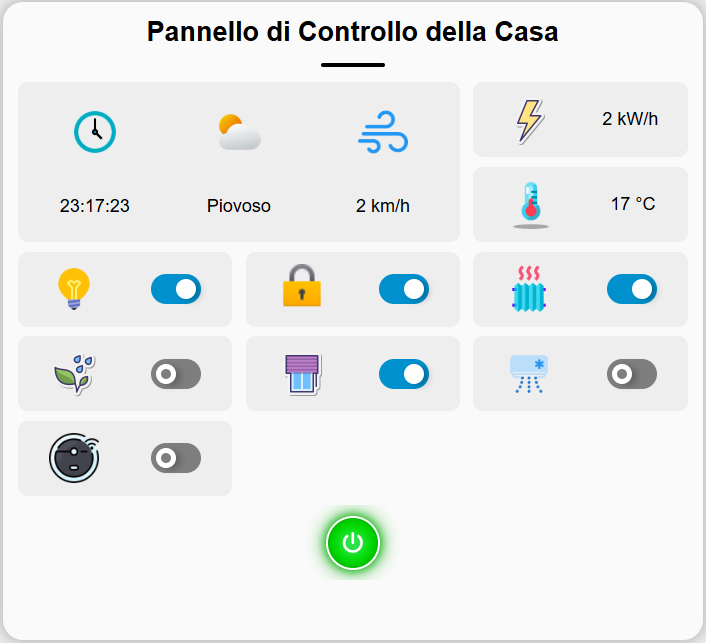
\includegraphics[width=0.6\linewidth]{image.png}

\section{Funzionalità}
\subsection*{Controllo Luci}
Permette di accendere o spegnere le luci. Cliccare sull’icona della lampadina per alternarne lo stato. Dal pannello si può decidere di nasconderle per una visualizzazione migliore della casa, oppure accenderle e spegnerle tutte contemporaneamente.

\subsection*{Stato Porte}
Visualizza se una porta è aperta o chiusa. Cliccando sull’icona della porta è possibile bloccarla oppure sbloccarla.

\subsection*{Monitoraggio Temperatura}
Mostra la temperatura interna ed esterna, fissa o simulata (sempre tramite l'utilizzo dei cookie).

\subsection*{Previsioni Meteo}
Visualizza informazioni come le condizioni meteo attuali e la velocità del vento.

\subsection*{Sistema di Irrigazione}
Permette di attivare o disattivare lo sprinkler esterno con un pulsante ON/OFF.

\subsection*{Gestione Roomba}
Permette di accendere o spegnere il Roomba, l'aspirapolvere robot.

\section{Guida Passo-Passo}

\begin{enumerate}
  \item Accedere alla cartella dell'interfaccia consegnata e aprire con il browser desiderato il file \textbf{index.html};
  \item Aggiungere i parametri iniziali della casa nel form (ricompare ogni giorno);
  \item Interagire con i bottoni per accendere/spegnere i dispositivi desiderati;
  \item Interagire con le stanze della casa per accederle singolarmente;
  \item Consultare i parametri come meteo, temperatura, ora, velocità vento, wattaggio.
\end{enumerate}

\section{Suggerimenti e Buone Pratiche}

\begin{itemize}
  \item Utilizzare browser aggiornati;
  \item Non accedere da più dispositivi contemporaneamente;
  \item Non modificare il codice se non si hanno competenze tecniche.
\end{itemize}

\section{Risoluzione dei Problemi}

\begin{tabular}{|p{5cm}|p{5cm}|p{5cm}|}
\hline
\textbf{Problema} & \textbf{Causa possibile} & \textbf{Soluzione} \\
\hline
L’interfaccia non si carica & File HTML non trovato & Verificare percorso o server \\
\hline
Le luci non rispondono & Errore JavaScript & Controllare la console del browser \\
\hline
Il meteo non si aggiorna & Mancanza di connessione API & Usare dati simulati o verificare la rete \\
\hline
Icone mancanti & File immagini assenti & Controllare la cartella \texttt{/img/} \\
\hline
\end{tabular}

\subsection{Contatti e Supporto}

Per assistenza tecnica o richieste relative al progetto, rivolgersi allo sviluppatore.


\end{document}
